\documentclass[aspectratio=169]{beamer}

% because we need to claim weird things
\newtheorem{claim}{Claim}
\newtheorem{defn}{Definition}
%\newtheorem{lemma}{Lemma}
\newtheorem{thm}{Theorem}
\newtheorem{vita}{Vit\ae}
\newtheorem{qotd}{Quote of the Day}

\usepackage{algorithm}
\usepackage{algpseudocode}
\usepackage{listings}
\usepackage{color}
\usepackage{graphics}
\usepackage{ulem}
\bibliographystyle{unsrt}

% background image
\usebackgroundtemplate%
{%
    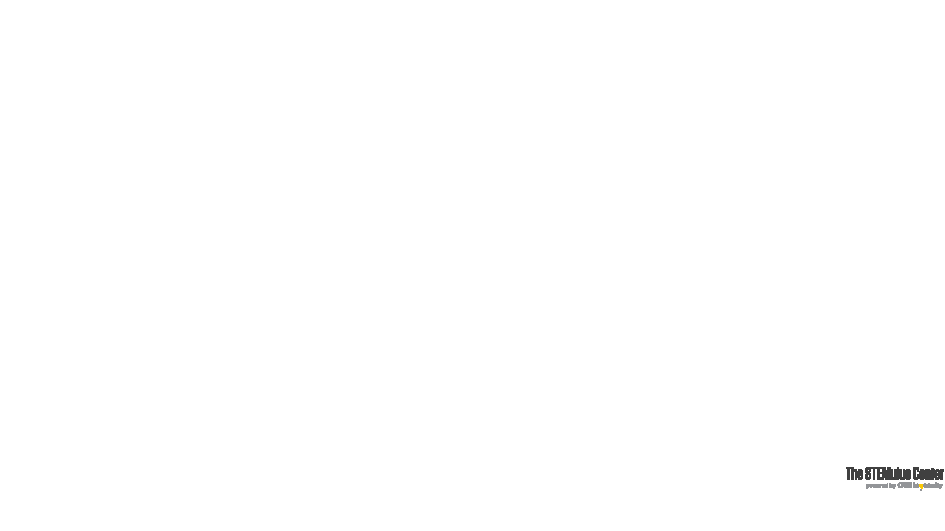
\includegraphics[width=\paperwidth,height=\paperheight]{../artifacts/stemulus.pdf}%
}
\setbeamertemplate{caption}[numbered]
\lstset{%
	breaklines=true,
	captionpos=b,
	frame=single,
	keepspaces=true,
	showstringspaces=false
}

% page numbers
\addtobeamertemplate{navigation symbols}{}{%
    \usebeamerfont{footline}%
    \usebeamercolor[fg]{footline}%
    \hspace{1em}%
    \insertframenumber/\inserttotalframenumber
}

% presentation header
\usetheme{Warsaw}
\title{Week 2: Object Oriented PHP}
\author{Dylan Lane McDonald}
\institute{CNM STEMulus Center\\Web Development with PHP}
\date{\today}

\begin{document}
\lstset{language=Java}
\begin{frame}
\titlepage
\end{frame}

\begin{frame}
\frametitle{Outline}
\tableofcontents
\end{frame}

\section{Introduction to Object Oriented Programming}
\subsection{Introduction to Object Oriented Programming}
\begin{frame}
\frametitle{Introduction to Object Oriented Programming}
\begin{defn}
\textbf{Object Oriented Programming} is a paradigm where all the actors in a program are modeled first and relations and behaviors are then implemented.
\end{defn}

\pause
\mbox{}\\
The fundamental shift from the imperative paradigm to the object oriented paradigm is in what you conceptualize first: namely, the actors. By contrast, the imperative paradigm conceptualizes the procedures and steps before conceptualizing the actors.
\end{frame}

\begin{frame}
\frametitle{What is an Object?}
\begin{defn}
An \textbf{object} is the nucleus of object oriented programming. Every object has a \emph{state} and \emph{behavior}. The state of an object is the data contained in the object. The behavior of the object are the \emph{methods} that contain code that manipulate and use the object.
\end{defn}

\pause
\mbox{}\\
In creating an object, one starts by first determining the state of the object; thus answering the question ``what is this object for?'' and then the behavior, which addresses the question ``what does this object do?'' This is the typical thought process when writing object oriented programs.
\end{frame}

\subsection{Encapsulation}
\begin{frame}
\frametitle{Encapsulation}
In object oriented programming, direct access to the object's state is problematic because it subverts the behavior. Therefore, the object's state is altered as a by product of its behavior.

\pause
\begin{defn}
\textbf{Encapsulation} is the prohibition of directly changing the object's state, and instead restricting state changes to methods defined by its behavior.
\end{defn}

\pause
The key way encapsulation works is by setting access levels to each member and method:
\begin{itemize}
	\item \textbf{public}: everyone can access (default)
	\item \textbf{protected}: only this object and child classes can access
	\item \textbf{private}: only this object can access
\end{itemize}
The general strategy is to make the object's state private and methods public.
\end{frame}

\subsection{Classes vs Objects}
\begin{frame}
\frametitle{Classes vs Objects}
As a developer, one writes a \textbf{class}. The end users see the results of the class, the \textbf{object}.

\begin{defn}
A \textbf{class} is a large code block that defines an object's state and behavior.
\end{defn}

\pause
\mbox{}\\
A useful metaphor would be to think as the class as a blueprint for how to make an object. The object is the tangible item \textbf{constructed} (or \textbf{instantiated}) using the class's schematic. This is a subtle distinction even experienced developers sometimes stumble on.
\end{frame}

\section{Programming in the New Paradigm}
\subsection{Getting Started}
\begin{frame}[fragile]
\frametitle{Writing Our First Class}
First, one defines the class's state and behavior. In this example, take a simple car class:
\begin{enumerate}
	\item \textbf{Model}: Any alpha numeric string
	\item \textbf{Cylinders}: Any positive, even integer
\end{enumerate}

Here, we have defined two items for the class's state and how we expect the state to behave.
\begin{lstlisting}[caption=The Car's State]
class Car {
   private $model;
   private $cylinders;
}
\end{lstlisting}
\end{frame}

\subsection{Accessor \& Mutator Methods}
\begin{frame}[fragile]
\frametitle{Accessor Methods}
Encapsulation does not directly allow one to read from the object's state. Therefore, we write \textbf{accessor methods}.
\begin{lstlisting}[caption=The Car's Accessor Methods]
class Car {
   public function getCylinders() {
      return($this->cylinders);
   }
   public function getModel() {
      return($this->model);
   }
}
\end{lstlisting}
\end{frame}

\begin{frame}
\frametitle{Have Some of \texttt{\$this}!}
In the previous slide, we saw a special keyword: \texttt{this}. The \texttt{this} keyword is a pointer to itself. The \texttt{this} keyword allows PHP to distinguish between a local variable in the function or a variable that is part of the object's state.

\pause
\mbox{}\\
The other operator we just saw is the \texttt{->} operator. This is actually pronounced the ``arrow operator''. The arrow operator signifies that the right hand side is a member of the class defined on the left hand side. This is the same as the . operator in JavaScript.
\[\underbrace{\texttt{\$this}}_{\substack{\text{pointer}\\\text{to}\\\text{myself}}}\underbrace{->}_{\substack{\text{member}\\\text{of}}}\underbrace{\texttt{model;}}_{\substack{\text{member}\\\text{I'm}\\\text{using}}}\]
\end{frame}

\begin{frame}[fragile]
\frametitle{Mutator Methods}
\begin{lstlisting}[caption=The Car's Mutator Methods]
class Car {
   public function setCylinders($newCylinders) {
      if($newCylinders <= 0 || $newCylinders % 2 != 0) {
         throw(new Exception("Cylinders must be even"));
      }
      $this->cylinders = $newCylinders;
   }
}
\end{lstlisting}
\end{frame}

\begin{frame}[fragile]
\frametitle{Mutator Functions}
\begin{lstlisting}[caption=The Car's Mutator Methods (cont)]
class Car {
   public function setModel($newModel) {
      $this->model = $newModel;
   }
}
\end{lstlisting}

Notice the syntax for throwing an exception. The \texttt{Exception} class is a system defined class in PHP and is ready-made for throwing a generic exception. The exception class in PHP is much more powerful to the throwing of Strings we did in JavaScript, and is much more akin to Java's \texttt{Exception} class.
\end{frame}

\subsection{Constructors \& Destructors}
\begin{frame}[fragile]
\frametitle{Constructors \& Destructors}
When an object is instantiated, the \textbf{constructor}, a method which sets the object's state, is executed. Conversely, when the object goes out of scope, the \textbf{destructor} is executed.
\begin{lstlisting}[caption=The Car's Constructor]
class Car {
   public function __construct($newModel, $newCylinders) {
      $this->setModel($newModel);
      $this->setCylinders($newCylinders);
   }
}
\end{lstlisting}
\end{frame}

\begin{frame}[fragile]
\frametitle{Creating An Object}
After the class is defined, it is ready to be created and used in your program. Listing 6 shows a simple example of how to use the class.
\begin{lstlisting}[caption=Creating a Car Object]
// the constructor is executed here
$honda = new Car("Honda", 6);
// change the object's state
$honda->setCylinders(8);
// access the object's state
echo $honda->getCylinders() . "<br />";
\end{lstlisting}
Note the use of the variable name \texttt{\$honda} at the beginning every time the object is used. This is required to properly reference the object.
\end{frame}
\end{document}
